\section{Problem Setting}

\begin{frame}{Problem Setting}
    Main objective:
    
    \begin{itemize}
        \item create an environmental indicator for \textbf{housing}.
    \end{itemize}
    
    \vspace{2.0 em}

    We aim to:

    \begin{itemize}
        \item focus on housing efficiency within England;
        \item assess accuracy of EPC ratings as an existing metric;
        \item describe trends in efficiency at a regional level.
    \end{itemize}
\end{frame}

\subsection{EPC? SAP?}

\begin{frame}{EPC? SAP?}
    Home energy efficiency and CO2 emissions assessed by 

    \begin{center}
        \textbf{S}tandard \textbf{A}ssessment \textbf{P}rocedure
    \end{center}

    which is used when awarding

    \begin{center}
        \textbf{E}nergy \textbf{P}erformance \textbf{C}ertificate(s)
    \end{center}

    to homes in the UK.
\end{frame}

\begin{frame}{EPC? SAP?}
    EPC certificates primarily focus on energy efficiency.

    \vspace{1.0 em}

    A SAP rating of 1 - 100 informs the band A - G as shown.

    \begin{figure}[H]
        \centering
        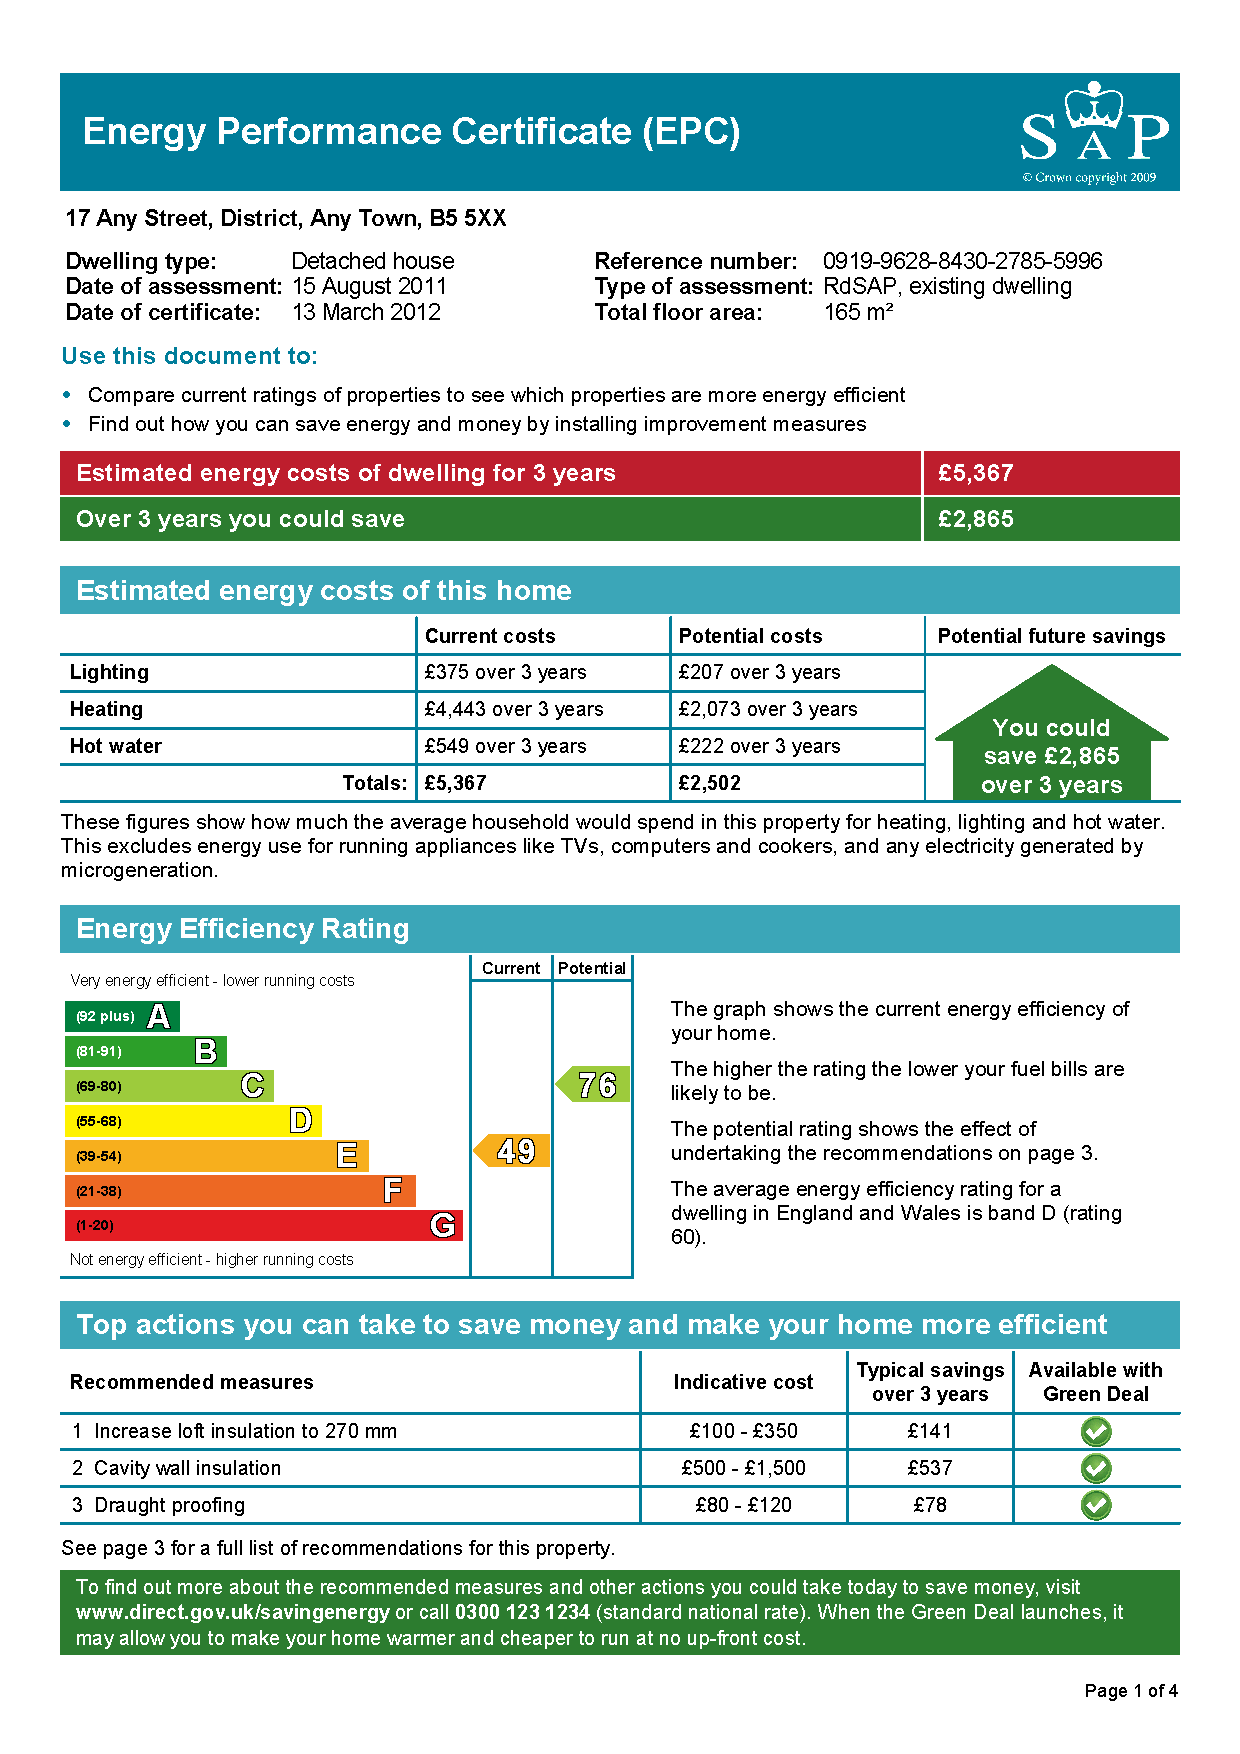
\includegraphics
            [trim = 0cm 8cm 0cm 15cm, clip, page = 1, width = \textwidth]
            {epc-sample-certificate} 
        \caption{Sample EPC certificate (Energy Efficiency Rating).}
        \label{fig:epc-sample-certificate-eer}
    \end{figure}
\end{frame}

\begin{frame}{EPC? SAP?}
    In addition, CO2 emissions highlighted via an environmental impact rating.
    	
    \begin{figure}[H]
        \centering
        \includegraphics
            [trim = 0cm 10.6cm 0cm 15.7cm, clip, page = 4, width = \textwidth]
            {epc-sample-certificate} 
        \caption{Sample EPC certificate (Energy Impact Rating).}
        \label{fig:epc-sample-certificate-eir}
    \end{figure}
\end{frame}

% Source (Information)
% > https://www.gov.uk/guidance/standard-assessment-procedure
% Source (Image)
% > https://assets.publishing.service.gov.uk/government/uploads/system/uploads/attachment_data/file/5996/2116821.pdf
